\section{Results}\label{sec:results}

\subsection{Predictive Outcomes Under Two Selection Objectives}

Figure~\ref{fig:paired_outcomes} reports held-out accuracy and MCC for the 20 model--optimizer cells. Each line connects a cell evaluated under the two fitness functions and is averaged over the same three seeds. Across cells, the descriptive macro mean test accuracy is 0.623 for MCC/$F_1$ fitness and 0.617 for accuracy fitness. The corresponding macro mean test MCC values are 0.247 and 0.235. These quantities summarize the available cells; they are not population estimates.

The result is informative because it rejects a simplistic expectation that selecting on validation accuracy must increase every held-out accuracy value. Some configurations improve under accuracy fitness, whereas others decline, and the corresponding MCC changes are likewise heterogeneous. The selection objective thus interacts with backbone and optimizer rather than imposing a uniform ordering.

\begin{figure}[htbp]
\centering
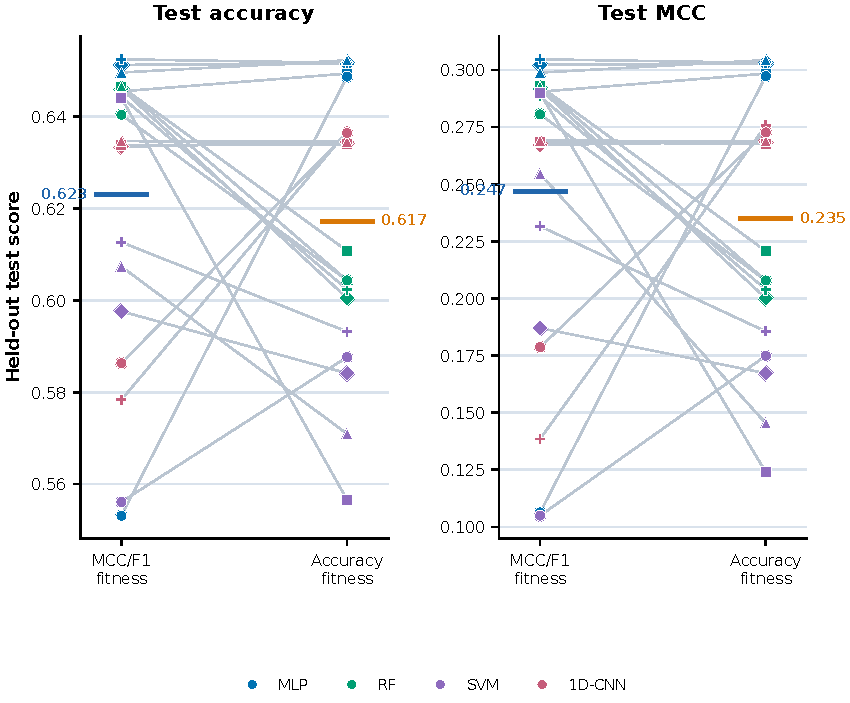
\includegraphics[width=0.96\linewidth]{figures/dual_fitness_paired_outcomes.pdf}
\caption{Held-out test outcomes under the two validation objectives. Each connection is one model--optimizer cell averaged over paired seeds 1--3. Colour denotes the model backbone; marker shape denotes the optimizer. Horizontal segments show macro means across the 20 cells.}
\label{fig:paired_outcomes}
\end{figure}

Figure~\ref{fig:delta_heatmaps} localizes the contrast by model and optimizer. Positive cells favour accuracy fitness and negative cells favour compound MCC/$F_1$ fitness. The heterogeneity reinforces the need to distinguish a selection objective from a reported test metric and motivates a larger common-seed study before making global superiority claims.

\begin{figure}[htbp]
\centering
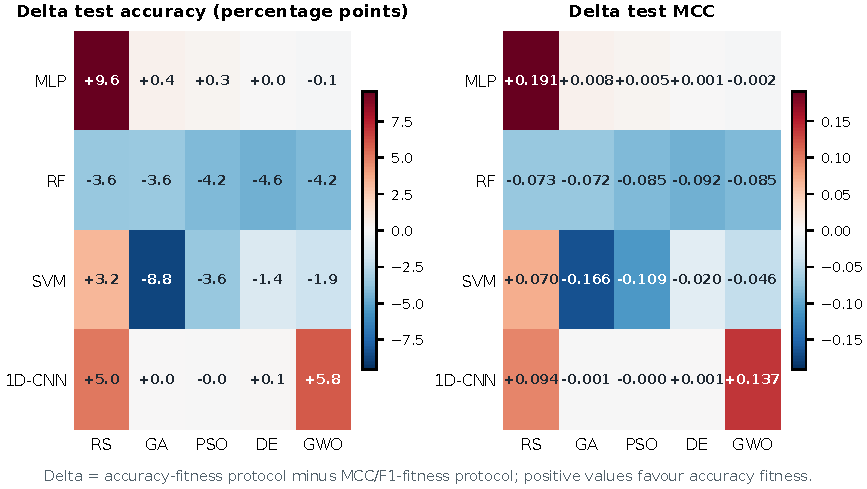
\includegraphics[width=0.96\linewidth]{figures/dual_fitness_delta_heatmaps.pdf}
\caption{Configuration-level difference between protocols (accuracy fitness minus MCC/$F_1$ fitness) on the locked test set. Left: accuracy in percentage points. Right: MCC in raw units.}
\label{fig:delta_heatmaps}
\end{figure}

\subsection{Search Dynamics}

Figure~\ref{fig:convergence} uses MLP as a reference backbone to visualize the objective being optimized. The left panel follows compound MCC/$F_1$ validation fitness, while the right panel follows validation accuracy. The vertical scales differ by construction and must not be interpreted as a direct score comparison. The trajectories show the progress of each optimizer under its assigned objective and make the distinction between the two experiments explicit.

\begin{figure}[htbp]
\centering
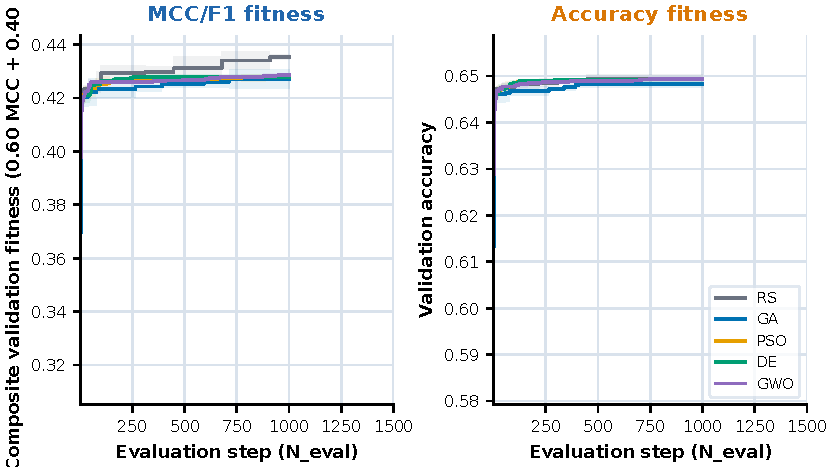
\includegraphics[width=0.96\linewidth]{figures/dual_fitness_convergence.pdf}
\caption{MLP convergence under the two validation objectives. Lines are means and shaded regions are $\pm1$ standard deviation across paired seeds 1--3. Left: compound MCC/$F_1$ fitness. Right: validation accuracy.}
\label{fig:convergence}
\end{figure}

\subsection{Exploratory Statistical Evidence}

Within Protocol A, the Friedman comparison across 15 matched optimizer--seed blocks identifies differences in test MCC among the four model backbones ($\chi^2=22.84$, $p=4.36\times10^{-5}$). Within Protocol B, the analogous test on accuracy is also significant ($\chi^2=42.92$, $p=2.56\times10^{-9}$), with MLP receiving mean rank 1.00. In Protocol B, Holm-adjusted MLP contrasts are significant against CNN, RF, and SVM ($p_{\mathrm{Holm}}=0.00194$ in each comparison).

These tests are exploratory and model-level. They do not test MCC/$F_1$ fitness against accuracy fitness, and their 15 blocks should not be confused with 15 independent market periods. Figure~\ref{fig:statistical_summary} makes this scope visible.

\begin{figure}[htbp]
\centering
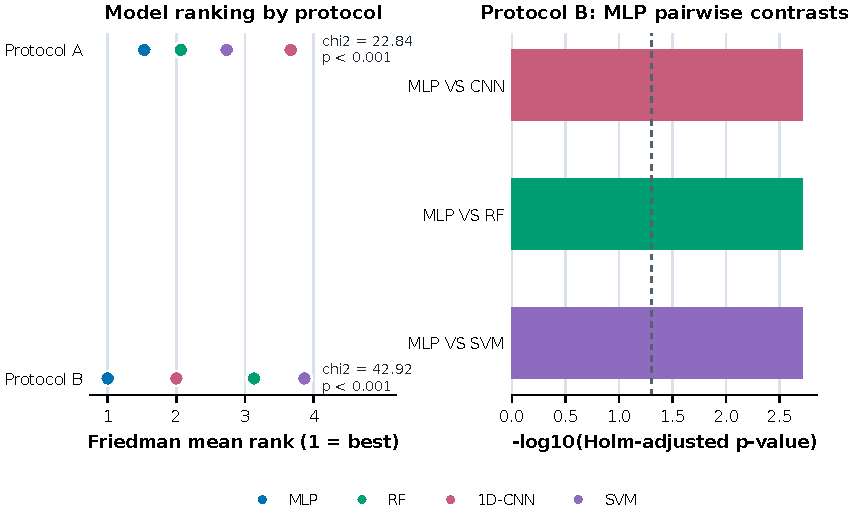
\includegraphics[width=0.96\linewidth]{figures/dual_fitness_statistical_summary.pdf}
\caption{Exploratory statistical evidence within each holdout protocol. Left: Friedman mean ranks across 15 matched optimizer--seed blocks (lower is better). Right: Holm-adjusted paired Wilcoxon evidence for MLP versus the other models under accuracy fitness; the dashed line denotes $\alpha=0.05$.}
\label{fig:statistical_summary}
\end{figure}

\subsection{Economic Evaluation}

The economic evaluation reveals a related but distinct ranking. Under MCC/$F_1$ fitness, RF has the largest mean total profit (26,465 points), but its Holm-adjusted profit contrasts are not significant. Under accuracy fitness, MLP has the largest mean total profit (27,737 points). MLP's profit advantage is significant against RF ($p_{\mathrm{Holm}}=0.00018$) and SVM ($p_{\mathrm{Holm}}=0.00305$), but not against CNN ($p_{\mathrm{Holm}}=0.169$). RF has the least negative mean drawdown under accuracy fitness ($-1,866$ points).

Figure~\ref{fig:economic_summary} shows why accuracy alone is insufficient for selection: total profit, dispersion, and drawdown do not always identify the same preferred configuration. The comparison is exploratory but establishes the economic endpoint absent from the precursor study.

\begin{figure}[htbp]
\centering
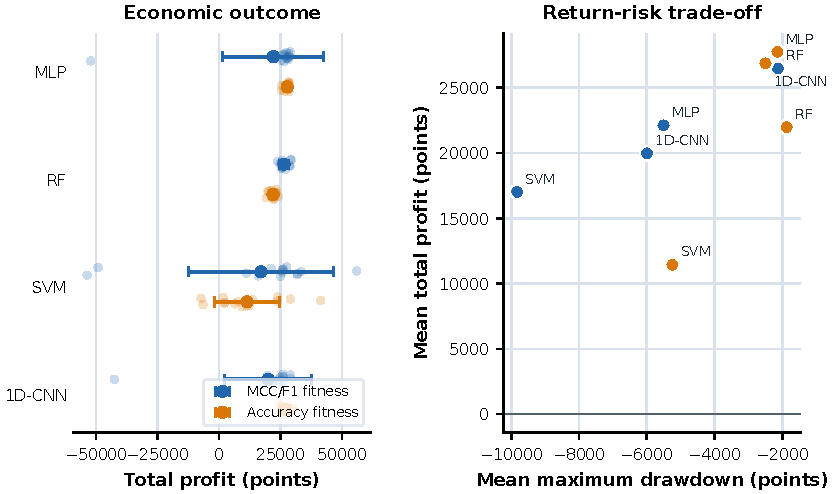
\includegraphics[width=0.96\linewidth]{figures/dual_fitness_economic_summary.pdf}
\caption{Exploratory economic evaluation on the locked test block. Left: total-profit observations and mean $\pm1$ standard deviation across 15 optimizer--seed blocks. Right: mean profit versus mean maximum drawdown; values farther right have less severe drawdown.}
\label{fig:economic_summary}
\end{figure}
